\documentclass[]{article}
\usepackage{lmodern}
\usepackage{amssymb,amsmath}
\usepackage{ifxetex,ifluatex}
\usepackage{fixltx2e} % provides \textsubscript
\ifnum 0\ifxetex 1\fi\ifluatex 1\fi=0 % if pdftex
  \usepackage[T1]{fontenc}
  \usepackage[utf8]{inputenc}
\else % if luatex or xelatex
  \ifxetex
    \usepackage{mathspec}
  \else
    \usepackage{fontspec}
  \fi
  \defaultfontfeatures{Ligatures=TeX,Scale=MatchLowercase}
\fi
% use upquote if available, for straight quotes in verbatim environments
\IfFileExists{upquote.sty}{\usepackage{upquote}}{}
% use microtype if available
\IfFileExists{microtype.sty}{%
\usepackage{microtype}
\UseMicrotypeSet[protrusion]{basicmath} % disable protrusion for tt fonts
}{}
\usepackage[margin=1in]{geometry}
\usepackage{hyperref}
\hypersetup{unicode=true,
            pdftitle={Dataset: Accidentes de avión acontecidos a nivel mundial},
            pdfauthor={Teguayco Gutiérrez González},
            pdfborder={0 0 0},
            breaklinks=true}
\urlstyle{same}  % don't use monospace font for urls
\usepackage{graphicx,grffile}
\makeatletter
\def\maxwidth{\ifdim\Gin@nat@width>\linewidth\linewidth\else\Gin@nat@width\fi}
\def\maxheight{\ifdim\Gin@nat@height>\textheight\textheight\else\Gin@nat@height\fi}
\makeatother
% Scale images if necessary, so that they will not overflow the page
% margins by default, and it is still possible to overwrite the defaults
% using explicit options in \includegraphics[width, height, ...]{}
\setkeys{Gin}{width=\maxwidth,height=\maxheight,keepaspectratio}
\IfFileExists{parskip.sty}{%
\usepackage{parskip}
}{% else
\setlength{\parindent}{0pt}
\setlength{\parskip}{6pt plus 2pt minus 1pt}
}
\setlength{\emergencystretch}{3em}  % prevent overfull lines
\providecommand{\tightlist}{%
  \setlength{\itemsep}{0pt}\setlength{\parskip}{0pt}}
\setcounter{secnumdepth}{0}
% Redefines (sub)paragraphs to behave more like sections
\ifx\paragraph\undefined\else
\let\oldparagraph\paragraph
\renewcommand{\paragraph}[1]{\oldparagraph{#1}\mbox{}}
\fi
\ifx\subparagraph\undefined\else
\let\oldsubparagraph\subparagraph
\renewcommand{\subparagraph}[1]{\oldsubparagraph{#1}\mbox{}}
\fi

%%% Use protect on footnotes to avoid problems with footnotes in titles
\let\rmarkdownfootnote\footnote%
\def\footnote{\protect\rmarkdownfootnote}

%%% Change title format to be more compact
\usepackage{titling}

% Create subtitle command for use in maketitle
\providecommand{\subtitle}[1]{
  \posttitle{
    \begin{center}\large#1\end{center}
    }
}

\setlength{\droptitle}{-2em}

  \title{Dataset: Pandemia Covid-19: Datos a nivel mundial}
    \pretitle{\vspace{\droptitle}\centering\huge}
  \posttitle{\par}
    \author{Raquel Gómez Pérez y Jorge Serra Planelles}
    \preauthor{\centering\large\emph}
  \postauthor{\par}
      \predate{\centering\large\emph}
  \postdate{\par}
    \date{14 de abril de 2020}

\usepackage[spanish]{babel}

\begin{document}
\maketitle

\hypertarget{descripcian}{%
\subsection{Descripción}\label{descripcian}}
El dataset generado contiene la información obtenida sobre la pandemia mundial Covid-19 a nivel de número de personas afectadas (infectadas, fallecidas...).

\hypertarget{imagen-identificativa}{%
\subsection{Representación gráfica}\label{imagen-identificativa}}
\subsection{}\label{imagen}
  	\begin{center}
  	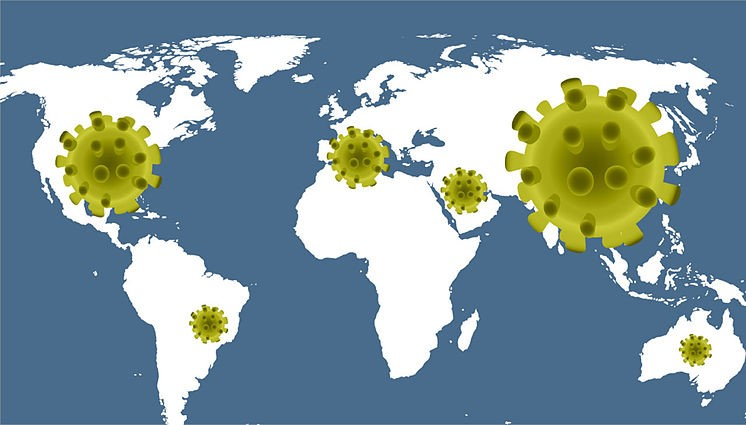
\includegraphics[width=0.7\textwidth]{covid}
	\end{center}
	
\hypertarget{contexto}{%
\subsection{Contexto}\label{contexto}}
Esta información se ha obtenido de tres páginas web:

\begin{itemize}
\tightlist
\item
  \textbf{https://www.worldometers.info/coronavirus/}: de esta web se ha obtenido la información total de todos los países y la información por estados de los Estados Unidos.\\
	Worldometers es una web que publica estadísticas del mundo en tiempo real. Por ejemplo cifras sobre población mundial, gobiernos y economía, sociedad y medios, medio ambiente, alimentos, agua, energía y salud. Actualmente, Worldometer es el proveedor de datos globales de COVID-19 para gobiernos e instituciones de todo el mundo.\\  
\item
  \textbf{https://covid19.isciii.es/}: de esta web se ha obtenido la información por regiones de España. en este caso solo existía información de casos totales.\\
  Esta web es propiedad del Instituto de Salud Carlos III (ISCIII) el cual es la referencia nacional e internacional en investigación biomédica y salud pública en España. Por tanto esta página recoge la notificación diaria de casos agregados de Covid-10 al Ministerio de sanidad.\\
\item
  \textbf{https://it.wikipedia.org/wiki/Pandemia\_di\_COVID-19\_del\_2020\_in\_Italia}: de esta web se ha obtenido la información por regiones de Italia.
	Wikipedia es una enciclopedia libre, políglota y editada de manera colaborativa, que tiene información de múltiples categorías, incluida la categoría 'Salud', en la cual estaría incluida esta información.\\  
\end{itemize}

\newpage

\hypertarget{contenido}{%
\subsection{Contenido}\label{contenido}}
Los campos que se han recogido en el dataset son los siguientes:

\begin{itemize}
\tightlist
\item
  \textbf{País}: país para el cual vamos a obtener los datos de la pandemia Covid-19.\\
\item
  \textbf{Región}: región del país al que corresponden los datos. En caso que los datos sean del total del pais en este campo aparecerá 'Total'.\\
\item
  \textbf{Casos totales}: número total de personas registradas portadoras del Covid-19.\\
\item
  \textbf{Fallecimientos}: número de personas fallecidas a causa del virus.\\
\item
  \textbf{Recuperados}: número de personas que han sido portadoras del virus y se han recuperado. \\
\item
  \textbf{Casos activos}: número de personas portadoras del virus actualmente (casos totales - fallecimientos - recuperados).\\
\item
  \textbf{Casos cerrados}: número de personas que han portado el virus pero no son casos activos actualmente (recuperados + fallecimientos).\\
\item
  \textbf{Fecha}: fecha en la cual se han actualizado los datos en formato DD/MM/YYYY hh:mm.
\end{itemize}

Esta información se ha recogido a nivel mundial, con datos totales de países, y a nivel más específico según regiones para los tres países con más casos actualmente: Estados Unidos, España e Italia. Se trata de datos totales desde que comenzó la expansión del virus hasta la última fecha de actualización indicada en el campo fecha.


\hypertarget{agradecimientos}{%
\subsection{Agradecimientos}\label{agradecimientos}}

En primer lugar agradecemos al equipo de Worldometer, un equipo internacional de desarrolladores, investigadores y voluntarios que tienen como objetivo de hacer que las estadísticas mundiales estén disponibles en un formato de reflexión y tiempo relevante para una amplia audiencia de todo el mundo.
Para el caso de Covid-19 recopilan datos de informes oficiales, directamente de los canales de comunicación del Gobierno o indirectamente, a través de fuentes de medios locales cuando se consideran confiables.\\
En segundo lugar a la comunidad de wikipedia, por recopilar tantos temas de interés de forma libre y colaborativa.\\
En tercer lugar al Instituto de Salud Carlos III, es la referencia nacional e internacional en investigación biomédica y salud pública en España. Es el Organismo Público de Investigación (OPI) del Gobierno encargado de financiar y llevar a cabo la investigación biomédica nacional. Depende del Ministerio de Ciencia, Innovación y Universidades, aunque también está adscrito al Ministerio de Sanidad, Consumo y Bienestar Social.


\hypertarget{inspiracian}{%
\subsection{Inspiración}\label{inspiracian}}

El contenido del dataset es un tema de interés mundial actualmente, debido a la crisis sanitaria por la que estamos pasando. Hay muchos aspectos que pueden analizarse con estos datos, tanto desde un punto de vista matemático y estadístico como en relación a su impacto en las decisiones que han tomado diversos gobiernos regionales o nacionales. El procesamiento de estos datos es importante para la adopción de medidas orientadas a la reducción del número de contagios, o a la ralentización de los mismos. También podría ser interesante para realizar modelos de predicción de la evolución del brote.

\hypertarget{licencia}{%
\subsection{Licencia}\label{licencia}}

La licencia escogida para este conjunto de datos es Released Under CC0: Public Domain License.
Es una licencia libre de derechos, permite la libertad total de reproducción para terceros. Escogería esta porque, en primer lugar, los datos que hemos obtenidos ya son públicos, por lo que no tendría sentido pedir más derechos sobre ellos que los de las fuentes de origen. Además, requerir una licencia más estricta podría hacer que un posible usuario de los datos se echará para atrás para evitar líos legales. En segundo lugar, son datos que tienen interés público y general, por lo que la libre distribución de los mismos es más beneficiosa.

\hypertarget{cadigo-fuente-y-dataset}{%
\subsection{Código fuente y dataset}\label{cadigo-fuente-y-dataset}}

Tanto el código fuente escrito para la extracción de datos como el
dataset generado pueden ser accedidos a través de
\href{https://github.com/raquel8893/Tipologia-PRA1}{este enlace}.

\hypertarget{recursos}{%
\subsection{Recursos}\label{recursos}}

\begin{enumerate}
\def\labelenumi{\arabic{enumi}.}
\tightlist
\item
Reitz, K. 2018. Requests-HTML: HTML Parsing for Humans. From: https://requests.readthedocs.io/projects/requests-html/en/latest/.\\
\item
Richardson, R. 2020. Beautiful Soup Documentation. From Crummy: https://www.crummy.com/software/BeautifulSoup/bs4/doc/.\\
\item
Schafer, C. 2017. Python Tutorial: Web Scraping with BeautifulSoup and Requests. From YouTube: https://www.youtube.com/watch?v=ng2o98k983k\&t=917s.\\
\item
Schafer, C. 2019. Python Tutorial: Web Scraping with Requests-HTML. From YouTube: https://www.youtube.com/watch?v=a6fIbtFB46g\&t=645s.\\
\item
Creative Commons. 2020. From: https://creativecommons.org/.\\

\end{enumerate}


\end{document}
